\subsubsection{Registration through the creation of a new myTaxiService account.}
			To accompany this diagram, read the Scenario \hyperref[sec:NormalCustomerRegistrationScenario]{S.1}.

				\begin{table}[htpb]
					\centering
					\label{tab:NormalCustomerRegistrationDiagramTable}
					\begin{tabularx}{\textwidth}{lp{9cm}}
						\hline
						\hline
							\textbf{Subject}
						& 
							\textbf{Description}\\
						\hline
							Actors	       &  Guest User, myTaxiService Application, myTaxiService Server\\
						\hline
							Preconditions  &  Guest User must not be already registered\\
						\hline
							Execution      &  1.~Guest User open the myTaxiService Application.\\
										   &  2.~Guest User taps on the "Sign Up as a Customer" button.\\
										   &  3.~myTaxiService Application shows the registration page.\\
										   &  4.~Guest User fills up the registration form.\\
										   &  5.~Guest User taps on the "Submit" button.\\
						\hline
							Postconditions &  The Guest User is now a Customer, he is registered in \\ 
										   &  the database and he's now logged in.\\
						\hline
							Exceptions     &  1.~The email regex is not optimal (no regex for email is optimal)\\
										   &  2.~The connection is lost or the Guest User doesn't complete\\ 
										   &     the registration clicking the button.\\
									
						\hline
						\hline
					\end{tabularx}
				\end{table}
				
				\begin{figure}[H]
					\centering
					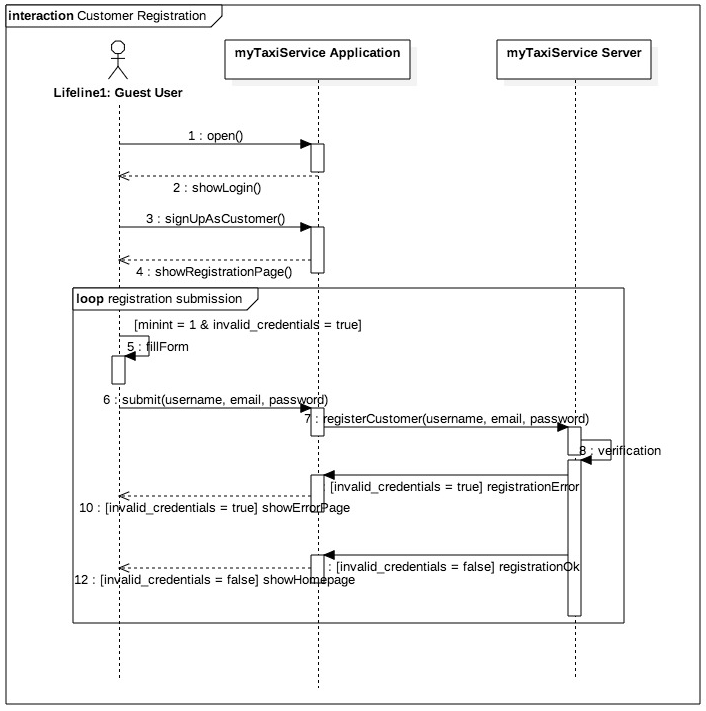
\includegraphics[width=\textwidth, scale=0.5]{IMG/InteractionDiagrams/CustomerRegistration_Normal.png}
					\caption{Customer Registration Interaction Diagram}\label{sec:FigureCustomerRegistration_Normal}
				\end{figure}